\section{Data Model}

% Task: How we broke down the Research question into parts
In this section, we will first demonstrate our general approach. We will show how we broke down the research question into smaller questions. Afterwards, we explain how we trained the individual models that were necessary to obtain our results. Then, we briefly evaluate the performance of our models.

\section*{Approach}
% State Problem: 

%todo: reformulate
The research question comes with one major issue: There is no real time \co emission data available.
To overcome this issue, we made several assumptions. We want to briefly present these assumptions here and explain how we approached the issue of predicting real time \co emissions, without having readily available emission data. The deviation from the usual emissions should then be used to find correlations with the impact of the COVID-19 pandemic. 

% Explain the proposed Solution: Real time indicators in combination with machine learning models. Divide country emissions into sectors. For each sector find a number of indicators, train them and predict 2020 emissions.
%todo: reformulate and check if the rest matches
After doing some literature research, we decided to follow an approach similar to \textit{Le Qu{\'e}r{\'e} et al}~\cite{LeQuere2020}. To describe our approach in a graphical way, we provide a data flow chart in \autoref{fig:model_pipeline}. The starting point of our analysis was the central question: How can we make as much use as possible from the EDGAR %todo: source, stated in data basis
dataset, which not only provides emission data per country, but also for the different sectors transport, other industrial combustion, other sectors and power industry? 

The central hypothesis is as follows: \emph{The emissions of a sector is a function of indicators that measures the activity or demand of a specific economic branch.} We limit the overall analysis to eight important regions: USA, EU, Russia, Brazil, India, China, Japan and Canada. As some indicators are not reliably updated, we consider the first six months of 2020 as the time period of interest.

%Prediction of 2020 emissions with and without the COVID-19 crisis
The goal was to find for each sector a method to extrapolate the general country trends from 2018, which is where the EDGAR data ends, to 2020. Here, we also tried to find out whether there exists a general seasonality for the emissions of a sector, and to find out which indicators work best to model the actual emission behavior. This is important as we don't want to confuse emission fluctuations in 2020 with general seasonal trends.

In order to predict the actual 2020 emissions, we need to find real time indicators for each sector such as activity, prices, et cetera in order to correlate them with the emissions from the past. Afterwards, the indicator can be used as a tool to predict the actual sector emissions.

%Calculate the emission drop and correlate it with COVID-19 impact
From the difference of the two values for 2020, we can estimate a total drop or increase in emissions per country. This can then be correlated with COVID-19 cases. Either we directly look at the correlation to see the general impact. Or we compare the drop or increase with the individual climate goal of the country. Doing the latter, we can estimate the degree that the crisis helped reaching the goal or not.

%Discussion and external factors
In summary, the strength of this approach lies in the validity of the indicators. As we take many different indicators into account, we minimize the risk of relying too much on a single data set.
%Discussion
Also, we do not have to consider some external influences, such as precipitation and other seasonal factors that impact the actual \co concentration. This is a strength of this approach, even though we would have liked to use the recently updated \co concentration data initially.



\begin{figure}[H]
	\centering
	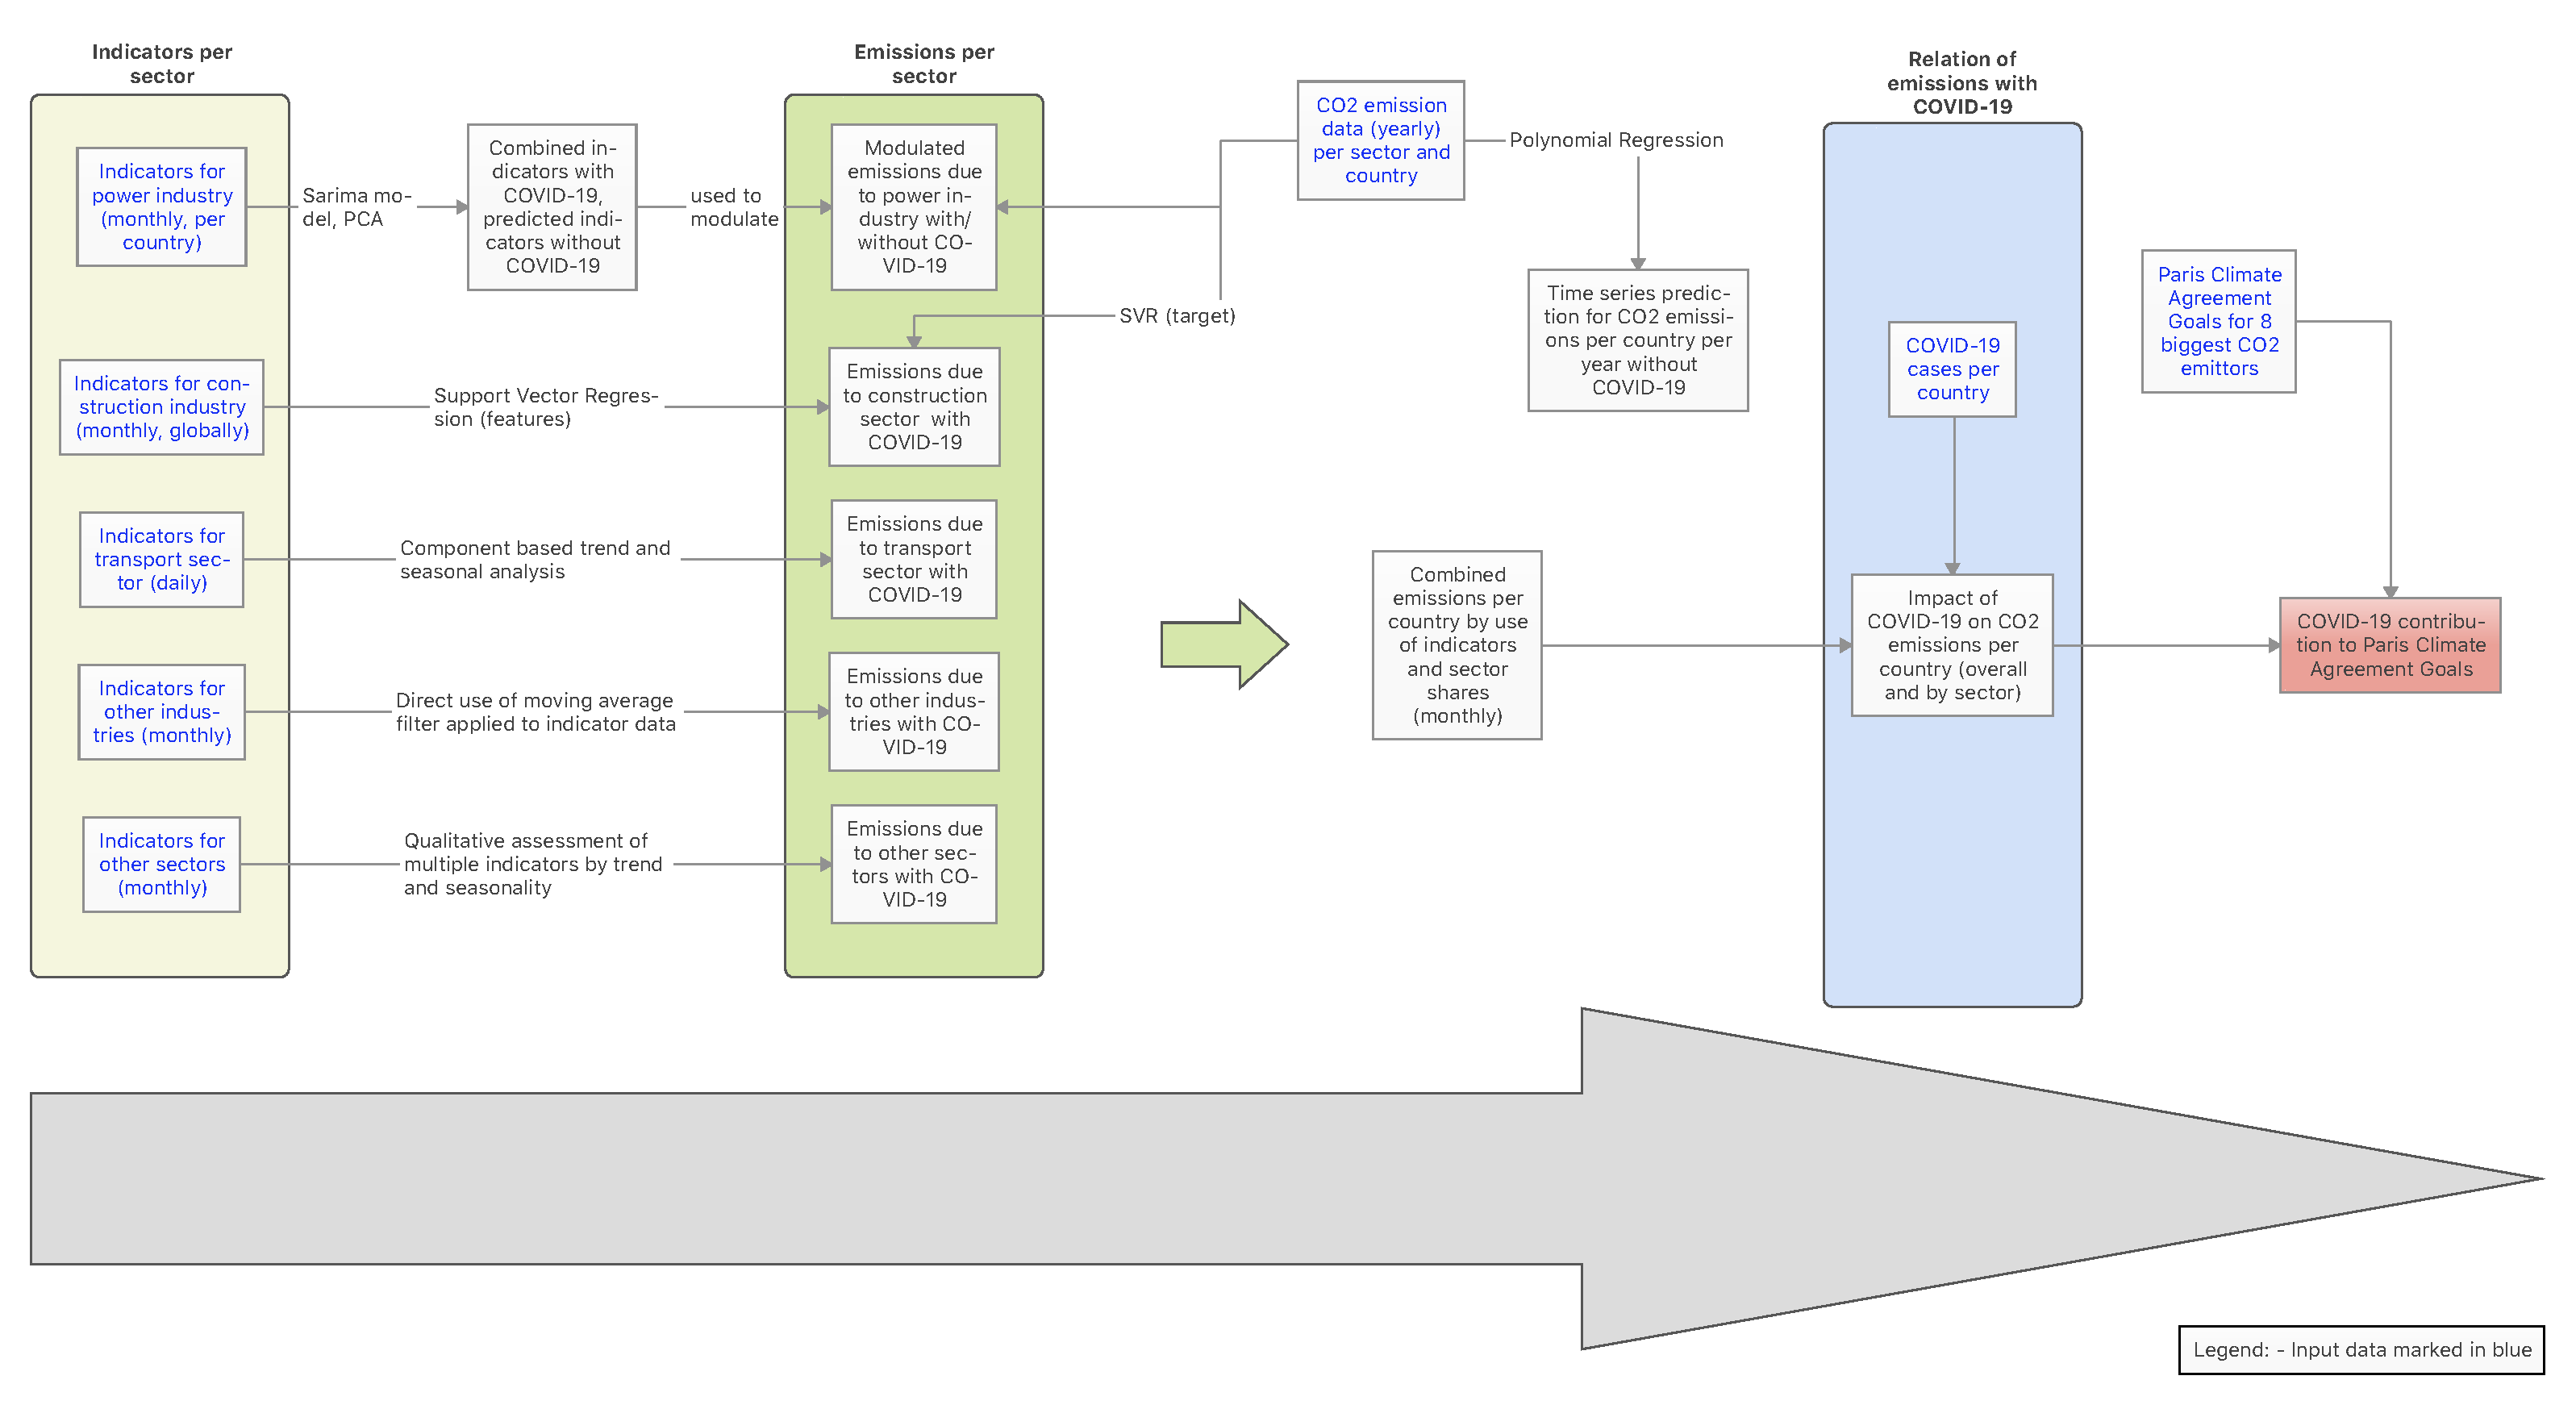
\includegraphics[width=1.45\linewidth, angle=90]{img/mock-up_frontend_pipeline_description.pdf}
	\caption{Depiction of the model pipeline. Input data is marked in blue.}
	\label{fig:model_pipeline}
\end{figure}




\section*{Model training}

%todo: Add Pipeline graphic from Max, should be full page, horizontally


\subsection*{Co2 prediction}

%todo: Explain CO2 prediction briefly
Our first idea was to get some datasets of indicators related to the corresponding sector with monthly data and up to date (at least up to May), that allowed us to predict how they would have behaved if the corona crisis would not have occurred. Then, after looking for the indicators, each sector prediction needed to be adapted according its indicators characteristics.


\subsection*{Sector summary}

%todo: For each sector: Indicator, ML Model, Evaluation, keep this short and concise
In the case of the power industry sector and the construction sector, the available data sets  allowed us to perform our original idea of predicting their normal behavior (without corona crisis) and compare it with the observed data. In the case of the transport sector and the other industries sector, it wasn't necessary to predict anything. For the other industries sector we only needed to adjust the seasonality of the indicators and normalize them. In the case of other sectors (mainly focused on agriculture) there was little data available and we were not able to compute a proper emission behavior. This is not optimal but since we can say that agriculture has seen little effect by the pandemic, we assume that there is no change.

\subsection*{Example: Power industry sector}

%todo: Select one example indicator (e.g. tranport) and explain how it was processed in more detail
We want to demonstrate how we computed the emission behavior for each sector by an example. We chose to do with the power industry sector.
For the power industry, we found four indicators: oil and power supply of the European countries and the brent and natural gas price. The first step was cleaning them so that they all started in 2008, normalizing them and separate them in different dictionaries. We separated them to differentiate between data before and after corona started; we set this date in December 2019. Then, we proceeded to search the indicator that was more correlated with the power industry emissions of each of the eight countries that produce the most \co emissions, assuming that they would behave in the same way after the start of the pandemic. With this, we trained a SARIMA model for each of the eight countries (seven countries and the European Union), where we predicted the behavior of the most correlated indicator.
In \autoref{fig:eu_prediction} we depict the prediction with and without the pandemic for the EU and summarize the resulting emission behavior for the power industry for all eight countries in \autoref{fig:power_ind_change_rate}.

Finally, we just compared the predicted versus the observed values of the indicators to generate a vector for each country with the fraction of \co emissions predicted between December and June.
Taking into account the lack of updated emissions data, we think that this is the best way to predict the drop in emissions if one is able to find good indicators.

\newpage

\begin{figure}[H]
	\centering
	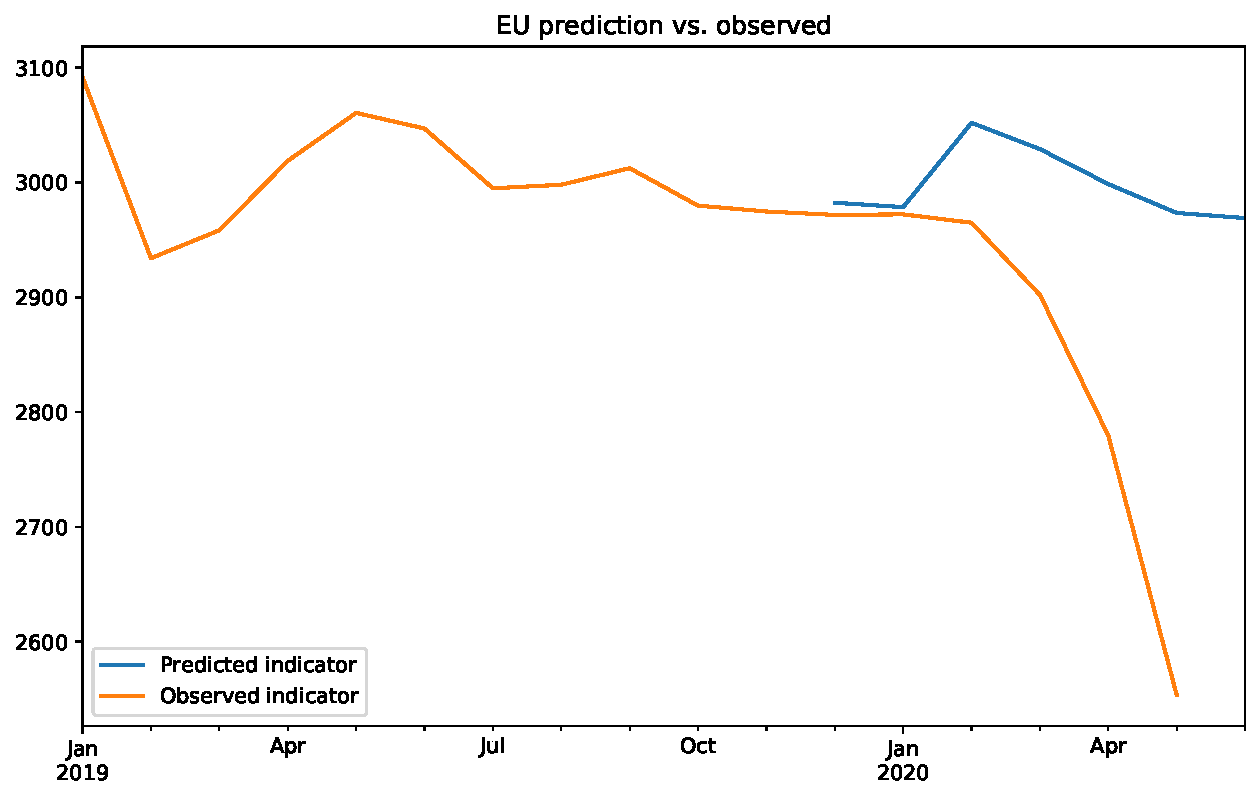
\includegraphics[width=0.85\textwidth]{img/EU_prediction.pdf}
	\caption{Predicted behaviour the best indicator for EU.}
	\label{fig:eu_prediction}
\end{figure}
%todo: Some text discussing it


%todo: Show resulting graph!!!
\begin{figure}[H]
	\centering
	\includegraphics[width=0.9\textwidth]{img/Power_industry_rate.pdf}
	\caption{Predicted behavior of the power industry for all countries considered. For most countries we see lowered emissions. For the EU we observe almost steady \co emissions.}
	\label{fig:power_ind_change_rate}
\end{figure}


\section*{Evaluation}

%todo: How valid are the results?
As previously discussed, it was crucial to have good indicators, this means having indicators highly correlated with the emissions of the corresponding sector.

% Task: Are the models good?
In the case of the power industry sector, we achieved high correlations for most of the countries. Probably with specific indicators for each country, correlations would have been better. This is complicated especially in the case of China, which has a very strict policy on sensitive data.
For the construction sector, the indicators used have different factors that affect them other than emissions. Therefore, the achieved correlations were not as good.
For the mobility sector, the dataset found already provided us the change in mobility which is, presumably the change in emissions. For the other industries sector, we had a similar case.
The emission behavior of the other sectors purely relies on our assumption that it will behave exactly as without the pandemic. This inflicts high uncertainties of course. For most countries, other sectors only contribute 10\% or less to the country's emission however. Therefore, it should not influence our final result as much.

